% $Id$
%
% Earth System Modeling Framework
% Copyright 2002-2022, University Corporation for Atmospheric Research, 
% Massachusetts Institute of Technology, Geophysical Fluid Dynamics 
% Laboratory, University of Michigan, National Centers for Environmental 
% Prediction, Los Alamos National Laboratory, Argonne National Laboratory, 
% NASA Goddard Space Flight Center.
% Licensed under the University of Illinois-NCSA License.

\section{Overview of Superstructure}

ESMF superstructure classes define an architecture for assembling
Earth system applications from modeling {\bf components}.  A component
may be defined in terms of the physical domain that it represents,
such as an atmosphere or sea ice model.  It may also be defined in terms
of a computational function, such as a data assimilation system.
Earth system research often requires that such components be {\bf coupled} 
together to create an application.  By coupling we mean the data 
transformations and, on parallel computing systems, data transfers, 
that are necessary to allow data from one component to be utilized by 
another.  ESMF offers regridding methods and other tools to simplify 
the organization and execution of inter-component data exchanges.  

In addition to components defined at the level of major physical 
domains and computational functions, components may be defined that 
represent smaller computational functions within larger components, 
such as the transformation of data between the physics and dynamics 
in a spectral atmosphere model, 
or the creation of nested higher resolution regions 
within a coarser grid.  The objective is to couple components at varying 
scales both flexibly and efficiently.  ESMF encourages a hierarchical
application structure, in which large components branch into 
smaller sub-components (see Figure \ref{fig:GEOS5}).  ESMF also makes 
it easier for the same component to be used in multiple contexts 
without changes to its source code.

\begin{center}  
\begin{tabular}{|p{6in}|}
\hline
\vspace{.01in}
{\bf Key Features} \\[.01in]
Modular, component-based architecture. \\
Hierarchical assembly of components into applications.\\
Use of components in multiple contexts without modification.\\
Sequential or concurrent component execution.\\
Single program, multiple datastream (SPMD) applications for 
maximum portability and reconfigurability.\\
Multiple program, multiple datastream (MPMD) option for 
flexibility.\\ [.03in] \hline
\end{tabular}
\end{center}

\subsection{Superstructure Classes}

There are a small number of classes in the ESMF superstructure:

\begin{itemize}
\item {\bf Component}  An ESMF component has two parts, one that is 
supplied by ESMF and one that is supplied by the user.  The
part that is supplied by the framework is an ESMF derived type that
is either a Gridded Component ({\bf GridComp}) or a Coupler 
Component ({\bf CplComp}).  A Gridded Component typically represents
a physical domain in which data is associated with one or more 
grids - for example, a sea ice model.  A Coupler Component 
arranges and executes data transformations and transfers between
one or more Gridded Components. Gridded Components and Coupler 
Components have standard methods, which include initialize, run,
and finalize.  These methods can be multi-phase.

The second part of an ESMF Component is user code, such as a
model or data assimilation system.  Users set entry points 
within their code so that it is callable by the framework.  
In practice, setting entry points means that within user code 
there are calls to ESMF methods that associate the name of a 
Fortran subroutine with a corresponding standard ESMF operation.  
For example, a user-written initialization routine called 
{\tt myOceanInit} might be associated with the standard 
initialize routine of an ESMF Gridded Component named ``myOcean'' 
that represents an ocean model.

\item {\bf State}  ESMF Components exchange information with other 
Components only through States.  A State is an ESMF derived
type that can contain Fields, FieldBundles, Arrays, ArrayBundles,
and other States.  A Component is associated with two States, an 
{\bf Import State} and an {\bf Export State}.  Its Import State 
holds the data that it receives from other Components.  
Its Export State contains data that it makes available to 
other Components. 

\end{itemize}

An ESMF coupled application typically involves a parent Gridded Component, 
two or more child Gridded Components and one or more Coupler 
Components. 

The parent Gridded Component is responsible for creating the child 
Gridded Components that are exchanging data, for creating the Coupler, 
for creating the necessary Import and Export States, and for 
setting up the desired sequencing.  The application's ``main'' routine
calls the parent Gridded Component's initialize, run, and finalize 
methods in order to execute the application.  For each of these
standard methods, the parent Gridded Component in turn calls the 
corresponding methods in the child Gridded Components and the 
Coupler Component.  For example, consider a simple coupled 
ocean/atmosphere simulation.  When the initialize method of the 
parent Gridded Component is called by the application, it in turn 
calls the initialize methods of its child atmosphere and ocean 
Gridded Components, and the initialize method of an 
ocean-to-atmosphere Coupler Component.  Figure \ref{fig:appunit}
shows this schematically.

\begin{center}
\begin{figure}
\caption{ESMF enables applications such as the atmospheric general
circulation model GEOS-5 to be structured hierarchically, and 
reconfigured and extended easily.  Each box in this diagram is an
ESMF Gridded Component.}
\label{fig:GEOS5}
\scalebox{0.9}{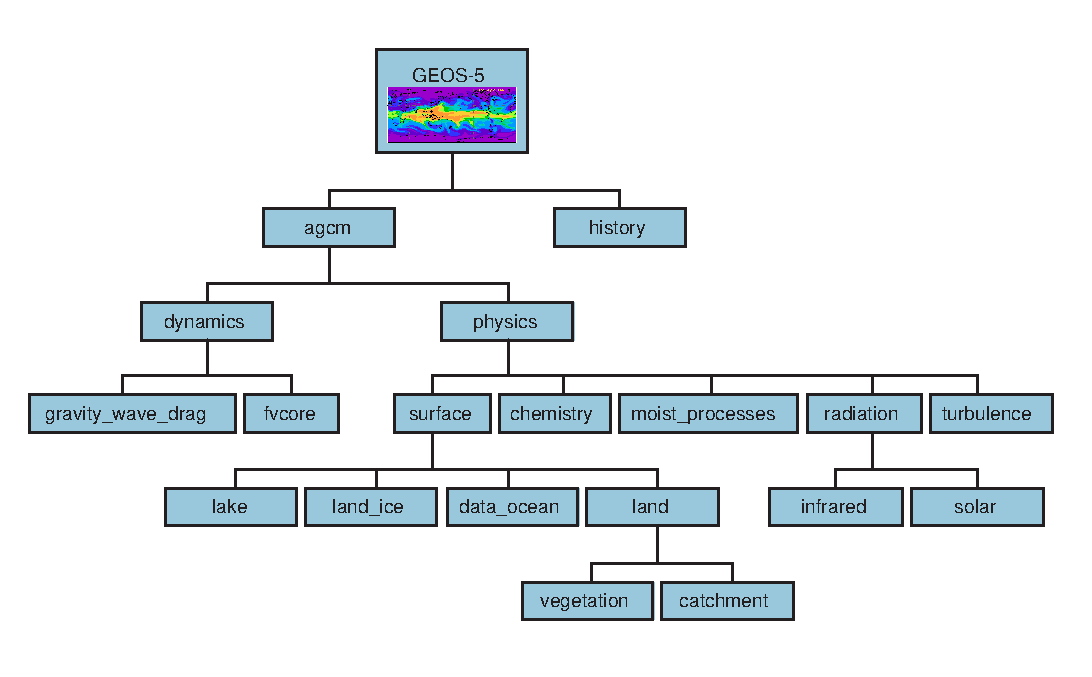
\includegraphics{ESMF_GEOS5}}
\end{figure}
\end{center}

\subsection{Hierarchical Creation of Components}
\label{sec:hierarchy}

Components are allocated computational resources in the form of
{\bf Persistent Execution Threads}, or {\bf PET}s.  A list of a Component's
PETs is contained in a structure called a {\bf Virtual Machine},
or {\bf VM}.  The VM also contains information about the topology and
characteristics of the underlying computer.
Components are created hierarchically, with parent Components creating
child Components and allocating some or all of their PETs to each one.
By default ESMF creates a new VM for each child Component, which 
allows Components to tailor their VM resources to match their needs.
In some cases, a child may want to share its parent's VM - ESMF
supports this, too.

A Gridded Component may exist across all the PETs in an application. 
A Gridded Component may also reside on a subset of PETs in an
application.  These PETs may wholly coincide with, be wholly contained
within, or wholly contain another Component.

\begin{center}
\begin{figure}
\caption{A call to a standard ESMF initialize (run, finalize) method
by a parent component triggers calls to initialize (run, finalize)
all of its child components.}
\label{fig:appunit}
\scalebox{1.0}{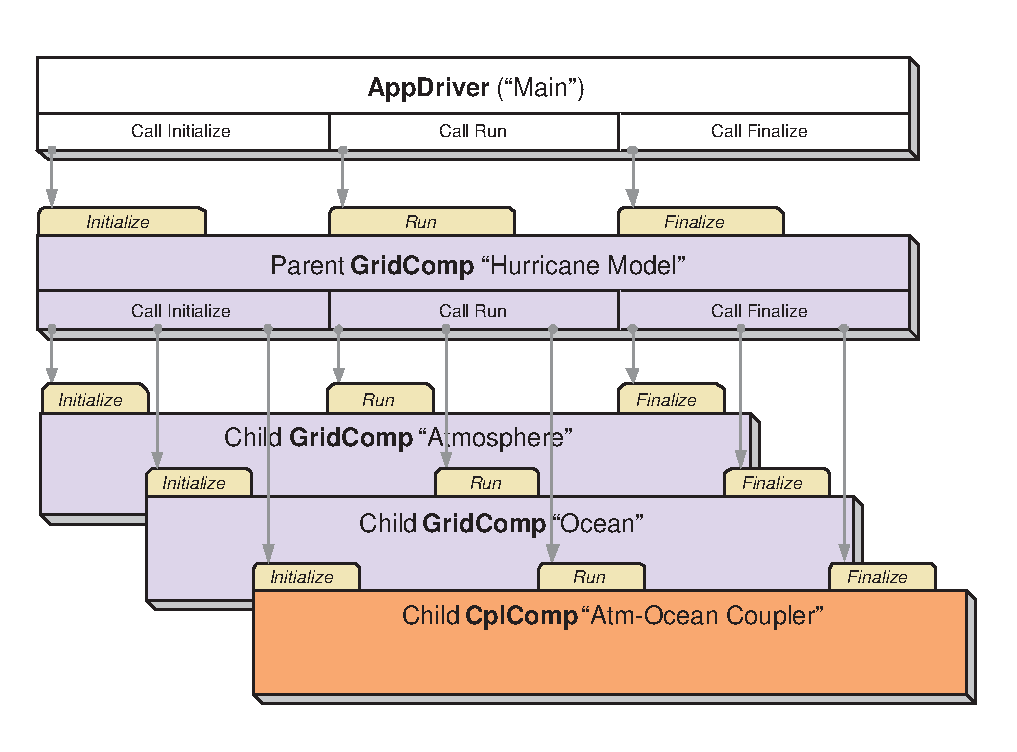
\includegraphics{ESMF_appunit}}
\end{figure}
\end{center}

\subsection{Sequential and Concurrent Execution of Components}
\label{sec:concurrency}

When a set of Gridded Components and a Coupler runs in sequence
on the same set of PETs the application is executing in a {\bf sequential}
mode. When Gridded Components are created and run on mutually exclusive
sets of PETs, and are coupled by a Coupler Component that extends over
the union of these sets, the mode of execution is {\bf concurrent}.

Figure \ref{fig:serial} illustrates a typical configuration for 
a simple coupled sequential
application, and Figure \ref{fig:concurrent} shows a possible 
configuration for the same application running in a concurrent mode.

Parent Components can select if and when to wait for concurrently
executing child Components, synchronizing only when required.

It is possible for ESMF applications to contain some Component sets
that are executing sequentially and others that are executing concurrently.
We might have, for example, atmosphere and land Components created
on the same subset of PETs, ocean and sea ice Components created on
the remainder of PETs, and a Coupler created across all the PETs in
the application.

\begin{center}
\begin{figure}
\caption{Schematic of the run method of a coupled application, with an
``Atmosphere'' and an ``Ocean'' Gridded Component running sequentially with 
an ``Atm-Ocean Coupler.''  The top-level ``Hurricane Model'' 
Gridded Component contains the sequencing information and time 
advancement loop.  The application driver, Coupler, and all Gridded Components 
are distributed over nine PETs.}
\label{fig:serial}
\scalebox{1.0}{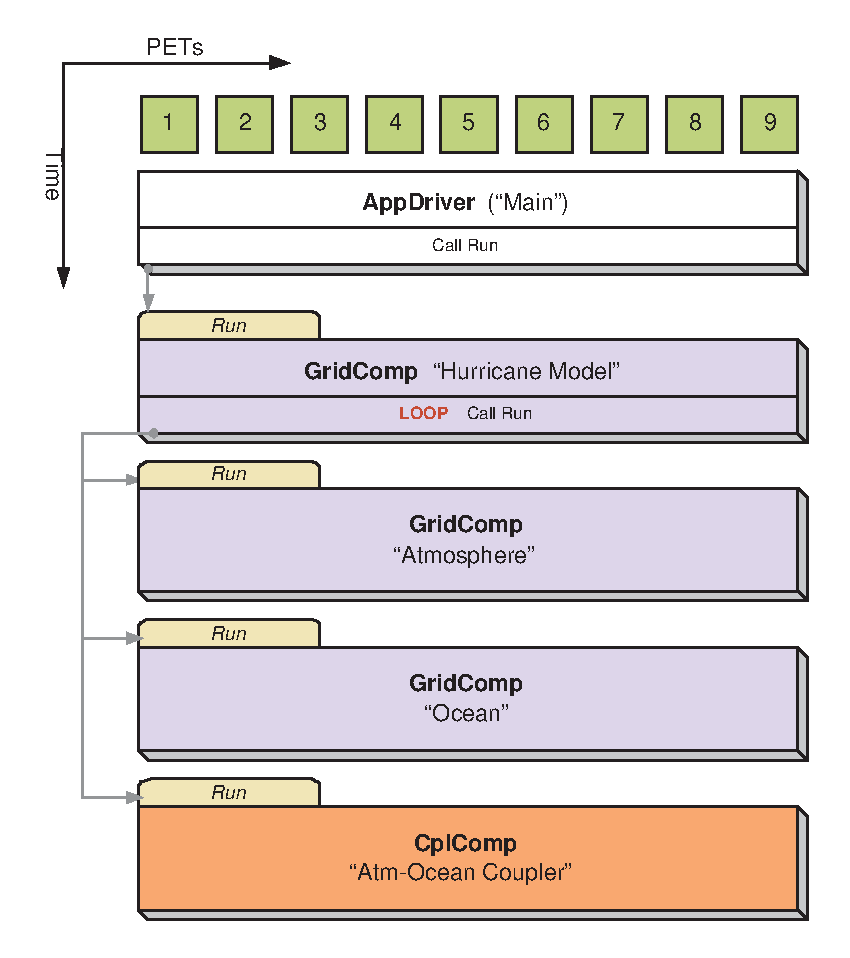
\includegraphics{ESMF_serial}}
\end{figure}
\end{center}

\begin{center}
\begin{figure}
\caption{Schematic of the run method of a coupled application, with an
``Atmosphere'' and an ``Ocean'' Gridded Component running concurrently with 
an ``Atm-Ocean Coupler.''  The top-level ``Hurricane Model'' 
Gridded Component contains the sequencing information and time 
advancement loop.  The application driver, Coupler, and top-level ``Hurricane
Model'' Gridded Component are distributed over nine PETs.  The
``Atmosphere'' Gridded Component is distributed over three PETs and
the ``Ocean'' Gridded Component is distributed over six PETs.}
\label{fig:concurrent}
\scalebox{1.0}{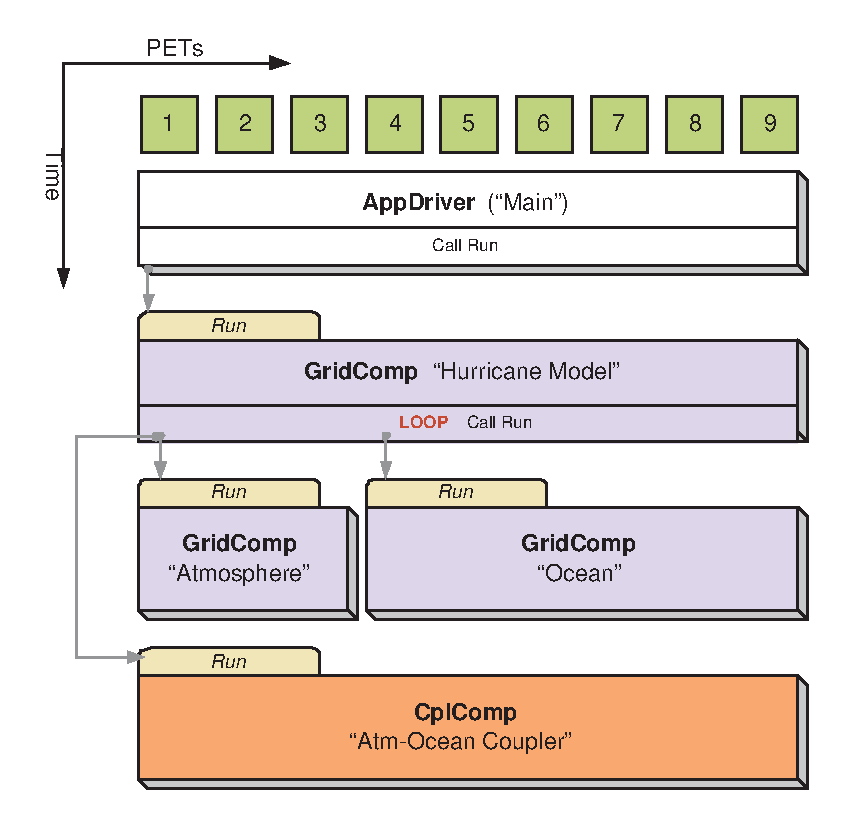
\includegraphics{ESMF_concurrent}}
\end{figure}
\end{center}

\subsection{Intra-Component Communication}
\label{sec:localcomm}

All data transfers within an ESMF application occur {\it within} a
component.  For example, a Gridded Component may contain halo updates.
Another example is that a Coupler Component may redistribute
data between two Gridded Components.  As a result,
the architecture of ESMF does not depend on any particular data
communication mechanism, and new communication schemes can be
introduced without affecting the overall structure of the application.

Since all data communication happens within a component, a Coupler
Component must be created on the union of the PETs of all
the Gridded Components that it couples.  

\subsection{Data Distribution and Scoping in Components}
\label{sec:scoping}

The scope of distributed objects is the VM of the currently 
executing Component.  For this reason, all
PETs in the current VM must make the same distributed object
creation calls.   When a Coupler Component running on a superset
of a Gridded Component's PETs needs to make communication calls
involving objects created by the Gridded Component,
an ESMF-supplied function called {\tt ESMF\_StateReconcile()} creates proxy
objects for those PETs that had no previous information about the
distributed objects.  Proxy objects contain no local data but
can be used in communication calls (such as regrid or redistribute)
to describe the remote source for data being moved to the current PET,
or to describe the remote destination for data being moved from the local PET.
Figure \ref{fig:reconcile} is a simple schematic that shows the 
sequence of events in a reconcile call.

\begin{center}
\begin{figure}
\caption{An {\tt ESMF\_StateReconcile()} call creates proxy 
objects for use in subsequent communication calls.  The reconcile 
call would normally be made during Coupler initialization.}
\label{fig:reconcile}
\scalebox{1.0}{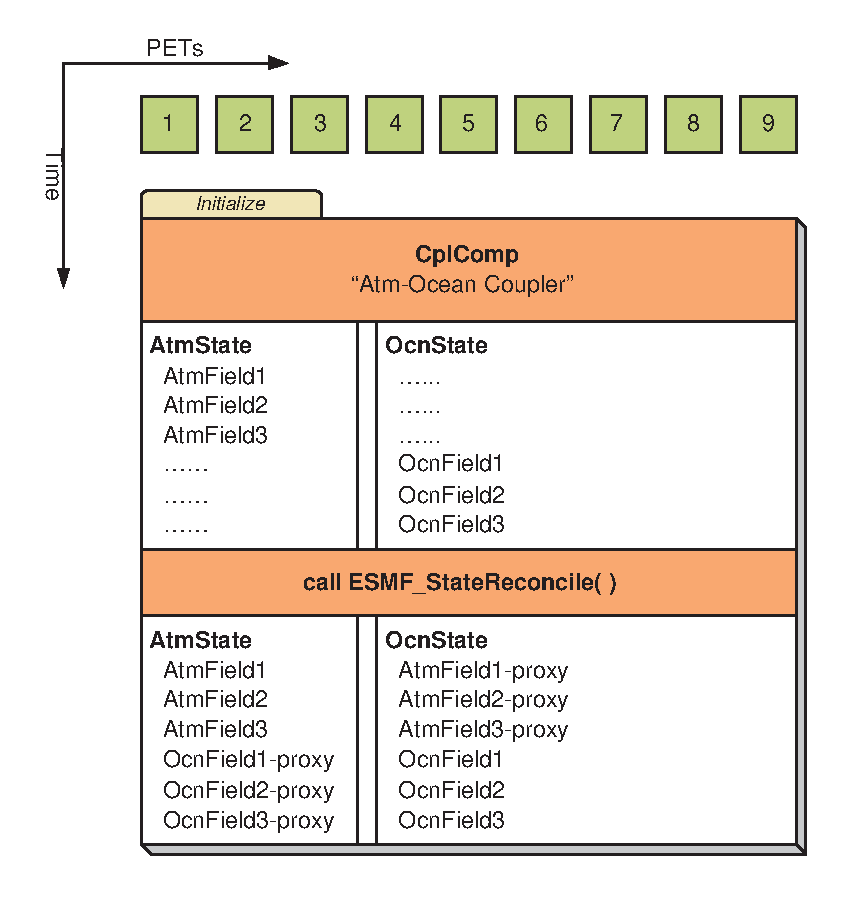
\includegraphics{ESMF_reconcile}}
\end{figure}
\end{center}

\subsection{Performance}
\label{sec:performance}

The ESMF design enables the user to configure ESMF
applications so that data is transferred directly from one component 
to another, without requiring that it be copied or sent to a different data
buffer as an interim step.  This is likely to be the most efficient way 
of performing inter-component coupling.  However, if desired, an 
application can also be configured so that data from a source component 
is sent to a distinct set of Coupler Component PETs for processing 
before being sent to its destination.

The ability to overlap computation with communication is essential for
performance.  When running with ESMF the user can initiate data 
sends during Gridded Component execution, as soon as the data is ready.
Computations can then proceed simultaneously with the data transfer.

\newpage
\subsection{Object Model}

The following is a simplified Unified Modeling Language (UML) diagram showing the relationships among
ESMF superstructure classes.  See Appendix A, {\it A Brief Introduction 
to UML}, for a translation table that lists the symbols in the diagram 
and their meaning.

\begin{center}
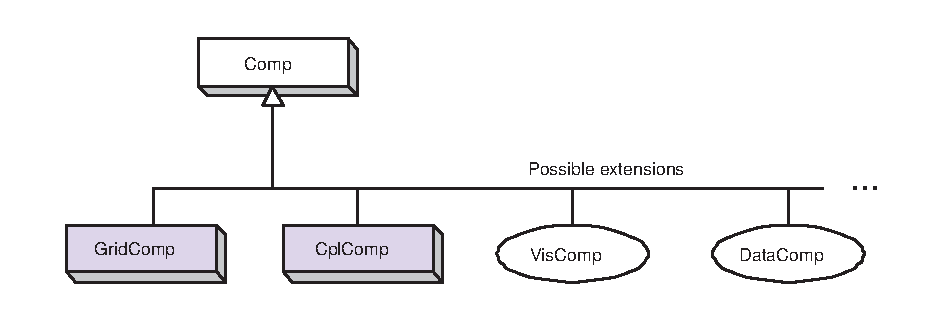
\includegraphics{Comp_obj}   
\end{center}



